\subsubsection{Creation of a Report}
Whenever the user wants to send a report of a parking violations to the authorities he has to follow what is visually described in the diagram below.
The user needs to insert a set of photos where a license plate is readable, and after confirming that the app has successfully read the license plate of the vehicles in the photos he should complete the form with the information required. At last he has to select if he wants to send an automatic or a manual ticket to the officers, after that the process is completed. If the automatic ticket option is selected, the AI and Computer Vision should identify a low degree of confidence.

\makebox[\textwidth][c]{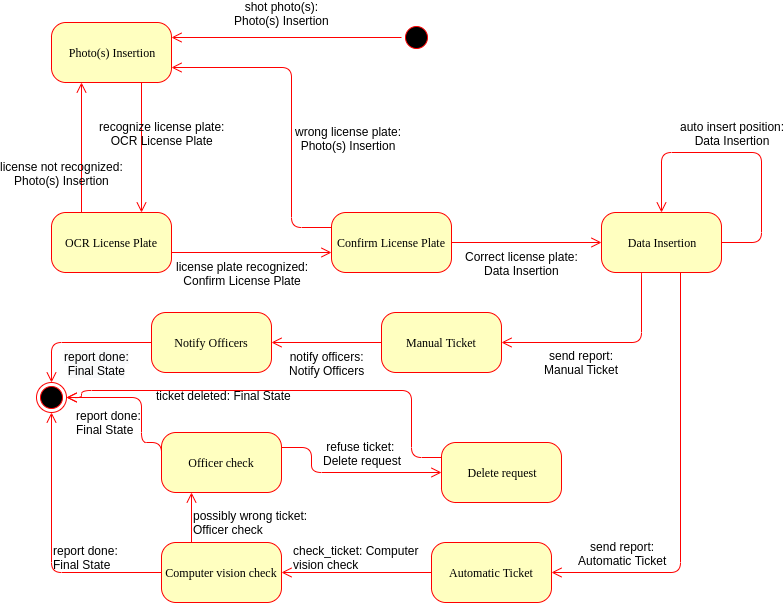
\includegraphics[width=1.2\textwidth]{diagrams/images/creationOfAReport}}
\clearpage
\subsubsection{Statistics Construction}
At the end of the day the statistics need to be updated in order to offer to the users and to the officers only recent, and therefore consistent, information.
When the servers will probably have the lowest load, so in the middle of the night, SafeStreets will at first retrieve the new data that are now present in the SafeStreets database. Once the complex queries have returned the new information the data needs to be aggregate and elaborate in order to exhibit the updated statistics to the costumers of SafeStreets. 
\\
\\
\\
\\
\\
\makebox[\textwidth][c]{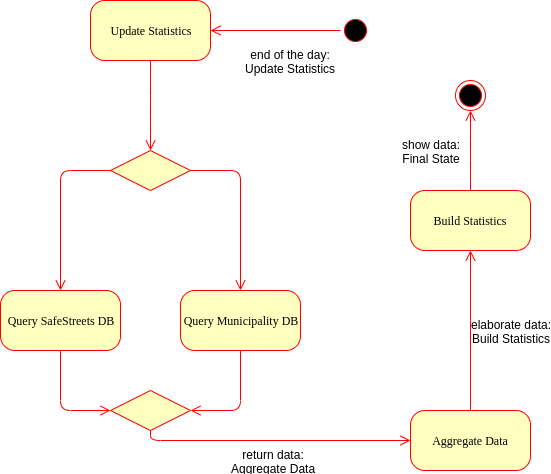
\includegraphics[width=1.0\textwidth]{diagrams/images/statisticsConstruction}}
\clearpage
\subsubsection{Data mining for Interventions}
At the end of the day as soon as the statistics are completed, the process of suggesting possible interventions needs to be executed. To do so, mining data using both SafeStreets data and municipality information on the accidents occurred in the city is necessary.
The flow is similar to the one for the statistics, since both needs to retrieve data, analyze it and produce some result with it.
After the process of computing information to suggest interventions in the city the authorities must be warned in order to actually intervene.
\\
\\
\\
\\
\\
\makebox[\textwidth][c]{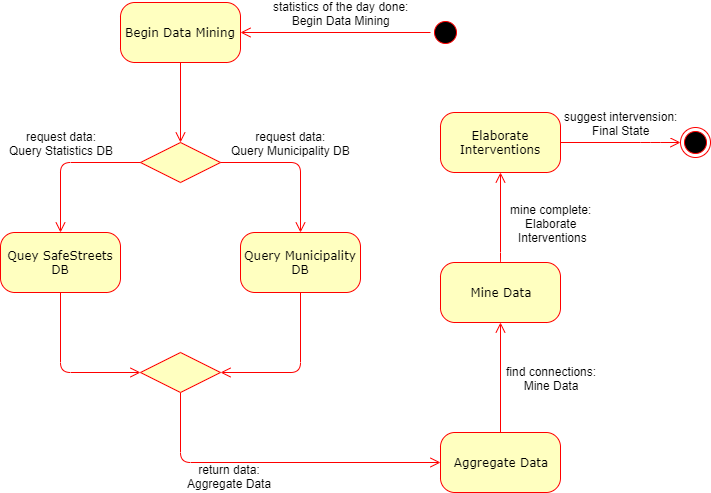
\includegraphics[width=1.2\textwidth]{diagrams/images/mineForInterventions}}
\clearpage